\chapter{Técnicas a reproducir}
\hrule  \vspace*{0.5cm}
%\section{Bases teóricas}
\section{Base de datos basado en Neo4j}
\subsection{Abstract}
Con el desarrollo de Internet, el crecimiento de los datos cinematográficos
rápidamente, la relación entre los datos de la película se vuelve más y
más complicado. Las relaciones entre películas, actores
y los escritores son información importante tanto para los productores de cine
y audiencias. El sitio web de datos de películas no solo necesita almacenar
vídeos de películas, también necesitan almacenar información sobre
directores, escritores, actores, etc.
Si tales datos se almacenan en una base de datos relacional, el
las conexiones entre diferentes tablas se pueden establecer a través de
llave. Sin embargo, cuando hay muchas relaciones, la base de datos relacional tradicional no solo tiene una gran cantidad de
redundancia de datos, pero también se vuelve difícil de actualizar
dinamicamente. Además, es difícil realizar consultas complejas
relaciones entre dos entidades. Por ejemplo, cuando
quieren saber si los principales productores de las dos películas
tienes una coproducción de otras películas, necesitas encontrar otras
películas producidas por los principales productores de las dos películas, y
luego analice si existe una intersección entre ellos.
Por lo tanto, la base de datos no relacional es una buena elección para
investigar y procesar datos de películas. Neo4j, que es un
excelente herramienta de base de datos de gráficos, almacena datos en forma de gráfico que puede representar objetos con nodos, aristas y propiedades \cite{lu2017analysis}.
En consecuencia, es adecuado para almacenar complejos y dinámicos
relaciones entre objetos de datos fílmicos, por lo que se desarrollará la recreación de la base de datos no relacional basada en grafos de Neo4j de DataFilm y su respectivo análisis.
\subsection{Neo4j}
Al momento de usar o crear bases de datos, las bases de datos relacionales han sido dominantes durante mucho tiempo.
Con la aplicación de Wed 2.0, el auge de las redes sociales, la dependencia y la complejidad de los datos internos aumentan gradualmente,
Cada vez surgen más problemas en las bases de datos relacionales. Luego,
apareció la base de datos basado en grafos.\\
En los últimos años ha habido una enorme cantidad de bases de datos basado en grafos de alto rendimient, existen multiples herramientas que trabajan con el diseño y la arquitectura de dicha base de datos entre ellas tenemos a Neo4j.
Esta herramienta en específico trabaja en la corriente principal de un software de código abierto basado en Jav, actualmente su kernel es un motor de gráficos muy rápido, con la recuperación de datos, con dos fases del envío, soporte para transacciones XA y otras características del producto de base de datos.
Neo4j es una base de datos orientada a la red, es decir, una base de datos integrada con motor de persistencia Java totalmente transaccional basado en disco que almacena datos estructurados en redes en lugar de tablas.
El lenguaje de esta herramienta es llamado Cypher el cual presenta sus propios comandos y formas de crear una base de datos con sus respectivos atributos.
En este modelo, los datos de dominio se expresan en un "espacio de nodos" la cual esta compuesta de: una red de nodos, relaciones y propiedades (pares clave-valor), en comparación con las tablas del modelo relacional, que trabajan con filas y columnas. Las relaciones son objetos de primera clase y pueden
también se tener  propiedades, revelando el contexto de cuales son los nodos con los que se interactúan. 
\subsection{Creación de la base de datos}
Para crear una base de datos basada en grafos debemos saber el funcionamiento de este y como empezar a crearla.La asociación es similar al borde en un grafo dirigido,El borde de esta base de datos consta de tres elementos: el nodo inicial, el nodo final y el tipo.
La orientación del borde aclara aún más la semántica y la
relación entre nodos.En la Figura \ref{fig:borde} vemos que los atributos de los nodos y las relaciones se pueden definir por clave-valor. Actores, directores,
escritores y películas son entidades diferentes cuando los datos de la película son almacenados, la base de datos de Neo4j no solo necesita almacenar entidades, sino también necesita almacenar las relaciones entre entidades.
\begin{figure}[H]
    \centering
    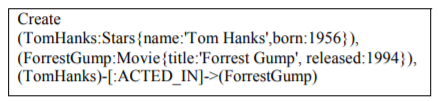
\includegraphics[scale=0.8]{Graficos/ejemplo.png}
    \caption{Ejemplo de la creación de un borde  \cite{lu2017analysis}.}
    \label{fig:borde}
\end{figure}
\subsection{Consultas y resultados}
En la Figura \ref{fig:grafo_bd} vemos el grafo de la película <The Green Mill> como el punto de partida, se crea una pequeña base de datos con 19 nodos y 19
relaciones como se muestra en la siguiente figura. En la figura tambien veremos que, el nodo de color verde significa que es un nodo de película,el amarillo significa que la etiqueta pertenece al nodo del actor,la etiqueta rosa significa que es un escritor, etiqueta azul significa que es un director, se utilizan diferentes colores para representar diferentes etiquetas y por ende diferentes tipos de nodos a construir.

\begin{figure}[H]
    \centering
    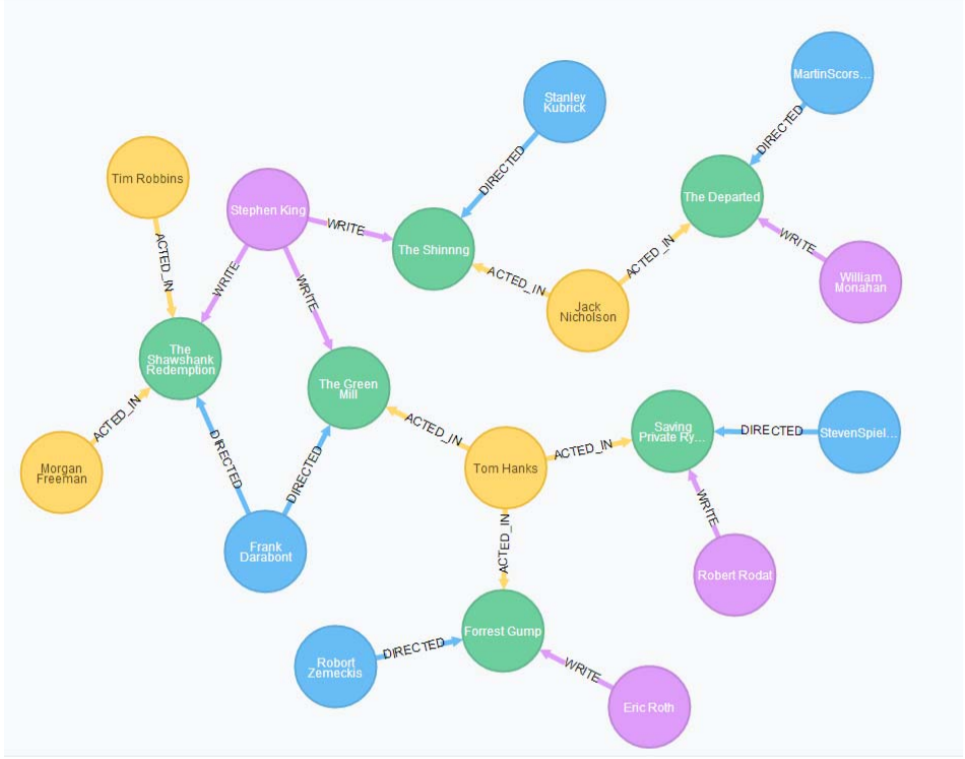
\includegraphics[scale=0.5]{Graficos/bd.png}
    \caption{Base de datos de películas en formato grafo \cite{lu2017analysis}.}
    \label{fig:grafo_bd}
\end{figure}
\newpage
Aquí hay un ejemplo,en la Figura \ref{fig:consulta} según el usuario ha visto la película.
<La redención Shawshank> y <Forrest Gump>, el sistema recomienda otras películas que se relacionen con las dos películas al usuario.
Por análisis encontramos que Tom Hanks actuó en <Forrest Gump>
y <The Green Mill>, el director Frank Darabont no solo
dirigió <THE Green Mill> pero también dirigió <The Shawshank
Redención>, por lo que encontramos la relación potencial entre la
película <Forrest Gump>, <The Shawshank Redemption> y
<The Green Mill>, por lo que podemos recomendar la película <The
Green Mill> al usuario. La siguiente es la consulta en el lenguaje Cypher muestra la consulta para este ejemplo.
\begin{figure}[H]
    \centering
    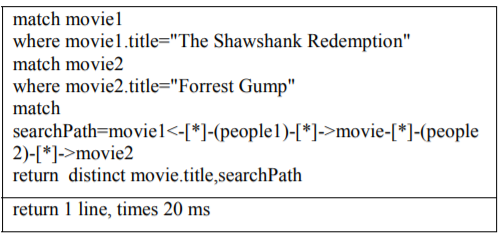
\includegraphics[scale=0.8]{Graficos/cypher1.png}
    \caption{Consulta en lenguaje Cypher \cite{lu2017analysis}.}
    \label{fig:consulta}
\end{figure}
Ya que la herramienta Neo4j nos brinda la opción de representar nuestra base de datos en una arquitectura de grafos usaremos esta opción para una mejor interpretación y después veremos el gráfico de dicha consulta en la Figura \ref{fig:rep} y como esta representado sus relaciones y nodos correspondientes.
\begin{figure}[H]
    \centering
    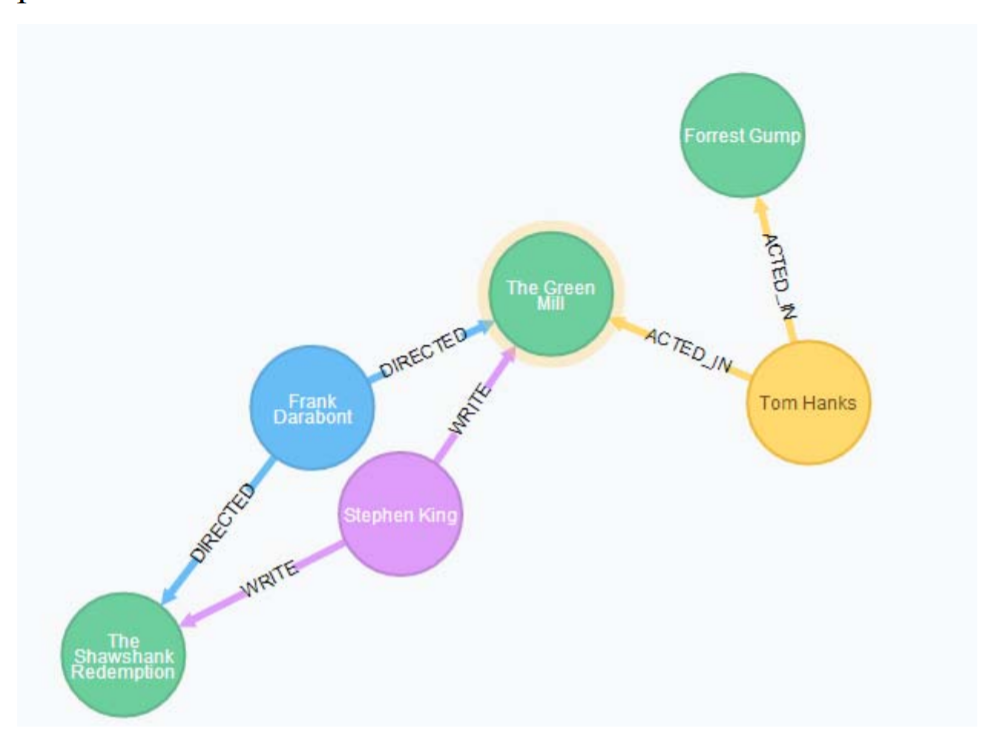
\includegraphics[scale=0.5]{Graficos/consultagraph.png}
    \caption{Representación en grafos de la consulta anterior \cite{lu2017analysis}.}
    \label{fig:rep}
\end{figure}
\section{Base de datos de investigación universitaria en Neo4j}
\subsection{Abstract}
En su mayoría, los datos relacionados con la investigación se modelan
usando una base de datos relacional optimizada para el proceso de transacciones, esto se debe a que es el tipo de base de datos mas común para dicho trabajo. En muchos casos, esta solución es eficaz y eficiente, lo suficiente como para responder consultas básicas e transacciones sencillas. Sin embargo, cuando los usuarios solicitan un análisis más detallado, más expansivo, con múltiples perspectivas y, a veces, un mayor análisis abstracto, la base de datos relacional lucha por proporcionar respuestas. Este estudio propone una base de datos basado en grafos de investigación implementado usando neo4j como la herramienta de creación para responder a los problemas.La base de datos permite que la
universidad pueda analizar el trabajo individual y colaborativo de los investigadores en conjunto de compañeros investigadores dentro y fuera de las
universidades. El estudio concluye que el gráfico de investigación que muestra que la implementación de la base de datos es más eficiente para responder
preguntas que la implementación de la base de datos relacional.
\subsection{Métodología}
Para la recolección de datos para la creación de nuestra base de datos basada en grafos se optó por evaluar las multiples fuentes de información consistentes y de buena procedencia que se pueden encontrar en la nube.
Entre aquellas podemos encontrar a Google Scholar.\\
Google Scholar es una plataforma denominado SINTA (Índice de Ciencia y Tecnología). Ristekbrin
(Ministerio de Investigación y Tecnología / Investigación Nacional y
Innovation Body) de Indonesia actualmente alberga SINTA.
SINTA utiliza datos de Google Scholar y otros
fuentes y luego calcula las capacidades de los investigadores,
instituciones y revistas en Indonesia. Los resultados son entonces
puesto a disposición del público de forma gratuita. Google Scholar
presenta ventajas que vale la pena destacar com los hechos que Google
Scholar ofrece referencias académicas más actualizadas. Existen
también API (interfaces de programación de aplicaciones) en varios
plataformas de programación creadas por desarrolladores que los investigadores,
profesionales y el público en general pueden utilizar para conectarse a
Google Scholar y recuperar datos de él de forma gratuita para académicos
con fines de investigación.
\subsection{Resultados}
Primeramente mostramos la creación de nuestra base de datos basada en grafos y usando como fuente de información la plataforma de google scholar.
La base de datos de grafos resultante de este estudio de caso consiste
de 12 etiquetas de nodo, 15 relaciones y 33 claves de propiedad.
La Tabla \ref{fig:tab_1} muestra todos los nombres de las etiquetas de los nodos, y la Tabla \ref{fig:tab_2} muestra los relación entre nodos.
\begin{figure}[H]
    \centering
    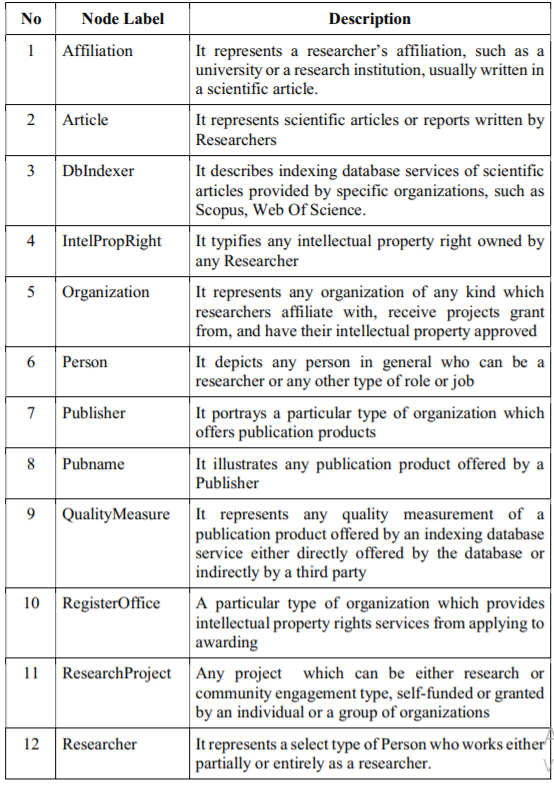
\includegraphics[scale=0.7]{Graficos/nodos.png}
    \caption{Nodos de la base de datos de investigación \cite{afandi2020university}.}
    \label{fig:tab_1}
\end{figure}
\begin{figure}[H]
    \centering
    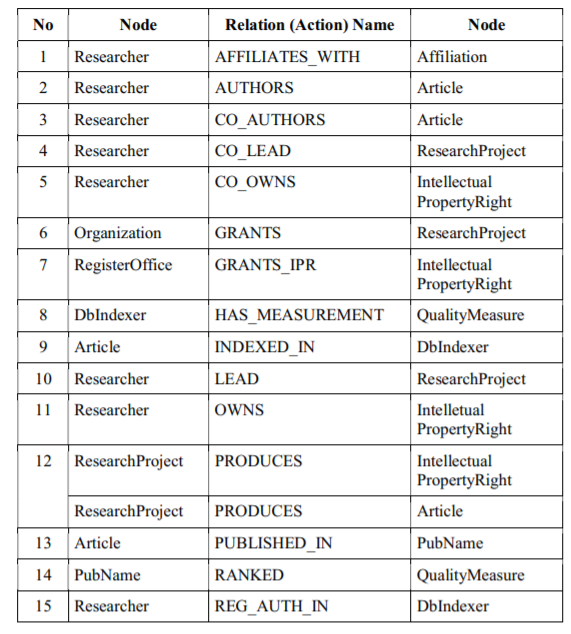
\includegraphics[scale=0.7]{Graficos/relaciones.png}
    \caption{Relaciones basado en los nodos de la base de datos de investigación \cite{afandi2020university}.}
    \label{fig:tab_2}
\end{figure}
La consulta de grafos escrita en Cypher como se muestra en la Figura \ref{fig:cypher}  es eficiente y simple. Podría decirse que puede ser formulado y realizado por trabajadores del conocimiento con menos experiencia que recibieron la formación previa y equipado con información tal como nodo y relación de nodo.
Además, la información visual que se muestra también es informativa.
y adecuado para diferentes niveles de espectadores, desde el conocimiento
trabajadores a ejecutivos.
 Una consulta más larga para responder a la misma pregunta en un relacional
es simulada en la Figura \ref{fig:sql}. La diferencia es clara. En
una base de datos relacional, el requisito debe ser muy explícito
por adelantado para que se traduzca correcta y cuidadosamente en consultas
antes de decidir qué tablas unir en qué columnas y
qué campos deben recuperarse. De hecho, requiere algunos
nivel de experiencia técnica para ejecutarlo.
\begin{figure}[H]
    \centering
    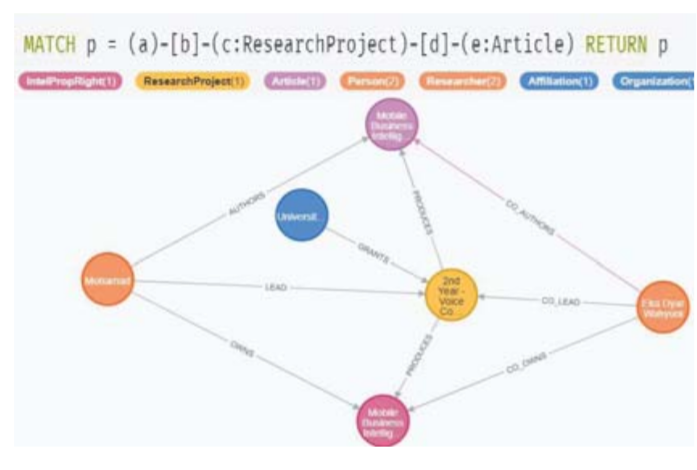
\includegraphics[scale=0.6]{Graficos/caso1.png}
    \caption{Consulta en lenguaje Cypher para la base de datos basada en grafos \cite{afandi2020university}.}
    \label{fig:cypher}
\end{figure}
\begin{figure}[H]
    \centering
    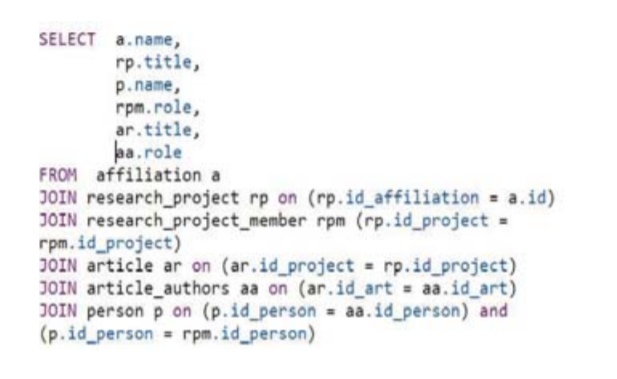
\includegraphics[scale=0.7]{Graficos/caso1_1.png}
    \caption{Consulta en SQL para la base de datos relacional \cite{afandi2020university}.}
    \label{fig:sql}
\end{figure}